\section{Modeler Integration}
\label{design:modeler_integration}

Looking at \autoref{image:2_tier}, we can see that the first interaction with the bootware is the call from the Modeler to the local bootware, which starts the bootstrapping process.
So in this section we are going to take a look at the integration between modeler and bootware in more detail.
The first question we face is: Why even divide the modeler and the local bootware?
Why not integrate the local bootware functionality into the modeler?
We go this route because we want the bootware to be as generic as possible.
The modeler in \autoref{image:2_tier} is not a specific modeler and in theory it should be possible to use the bootware with any modeler (and any workflow middleware) without too much modification.
So, by keeping the bootware as a separate generic component and only implementing a small, modeler specific adapter, we are able to support different environments without changing the core bootware components.
We call this abstract concept the bootware adapter, as shown in \autoref{image:modeler_plugin}.

In \autoref{requirements} we mentioned that the bootware should hook into the already existing deploy process in the modeler.
How this deployment process works depends on the actual modeler that is used, so at the moment, we can not say how exactly we can integrate in this process.
Specific integration details for our modeler, the SimTech Modeler, will be discussed in \autoref{implementation:modeler_integration}.
We know however what needs to happen in the bootware adapter to get the bootstrapping process going.

\begin{figure}[!htbp]
	\centering
	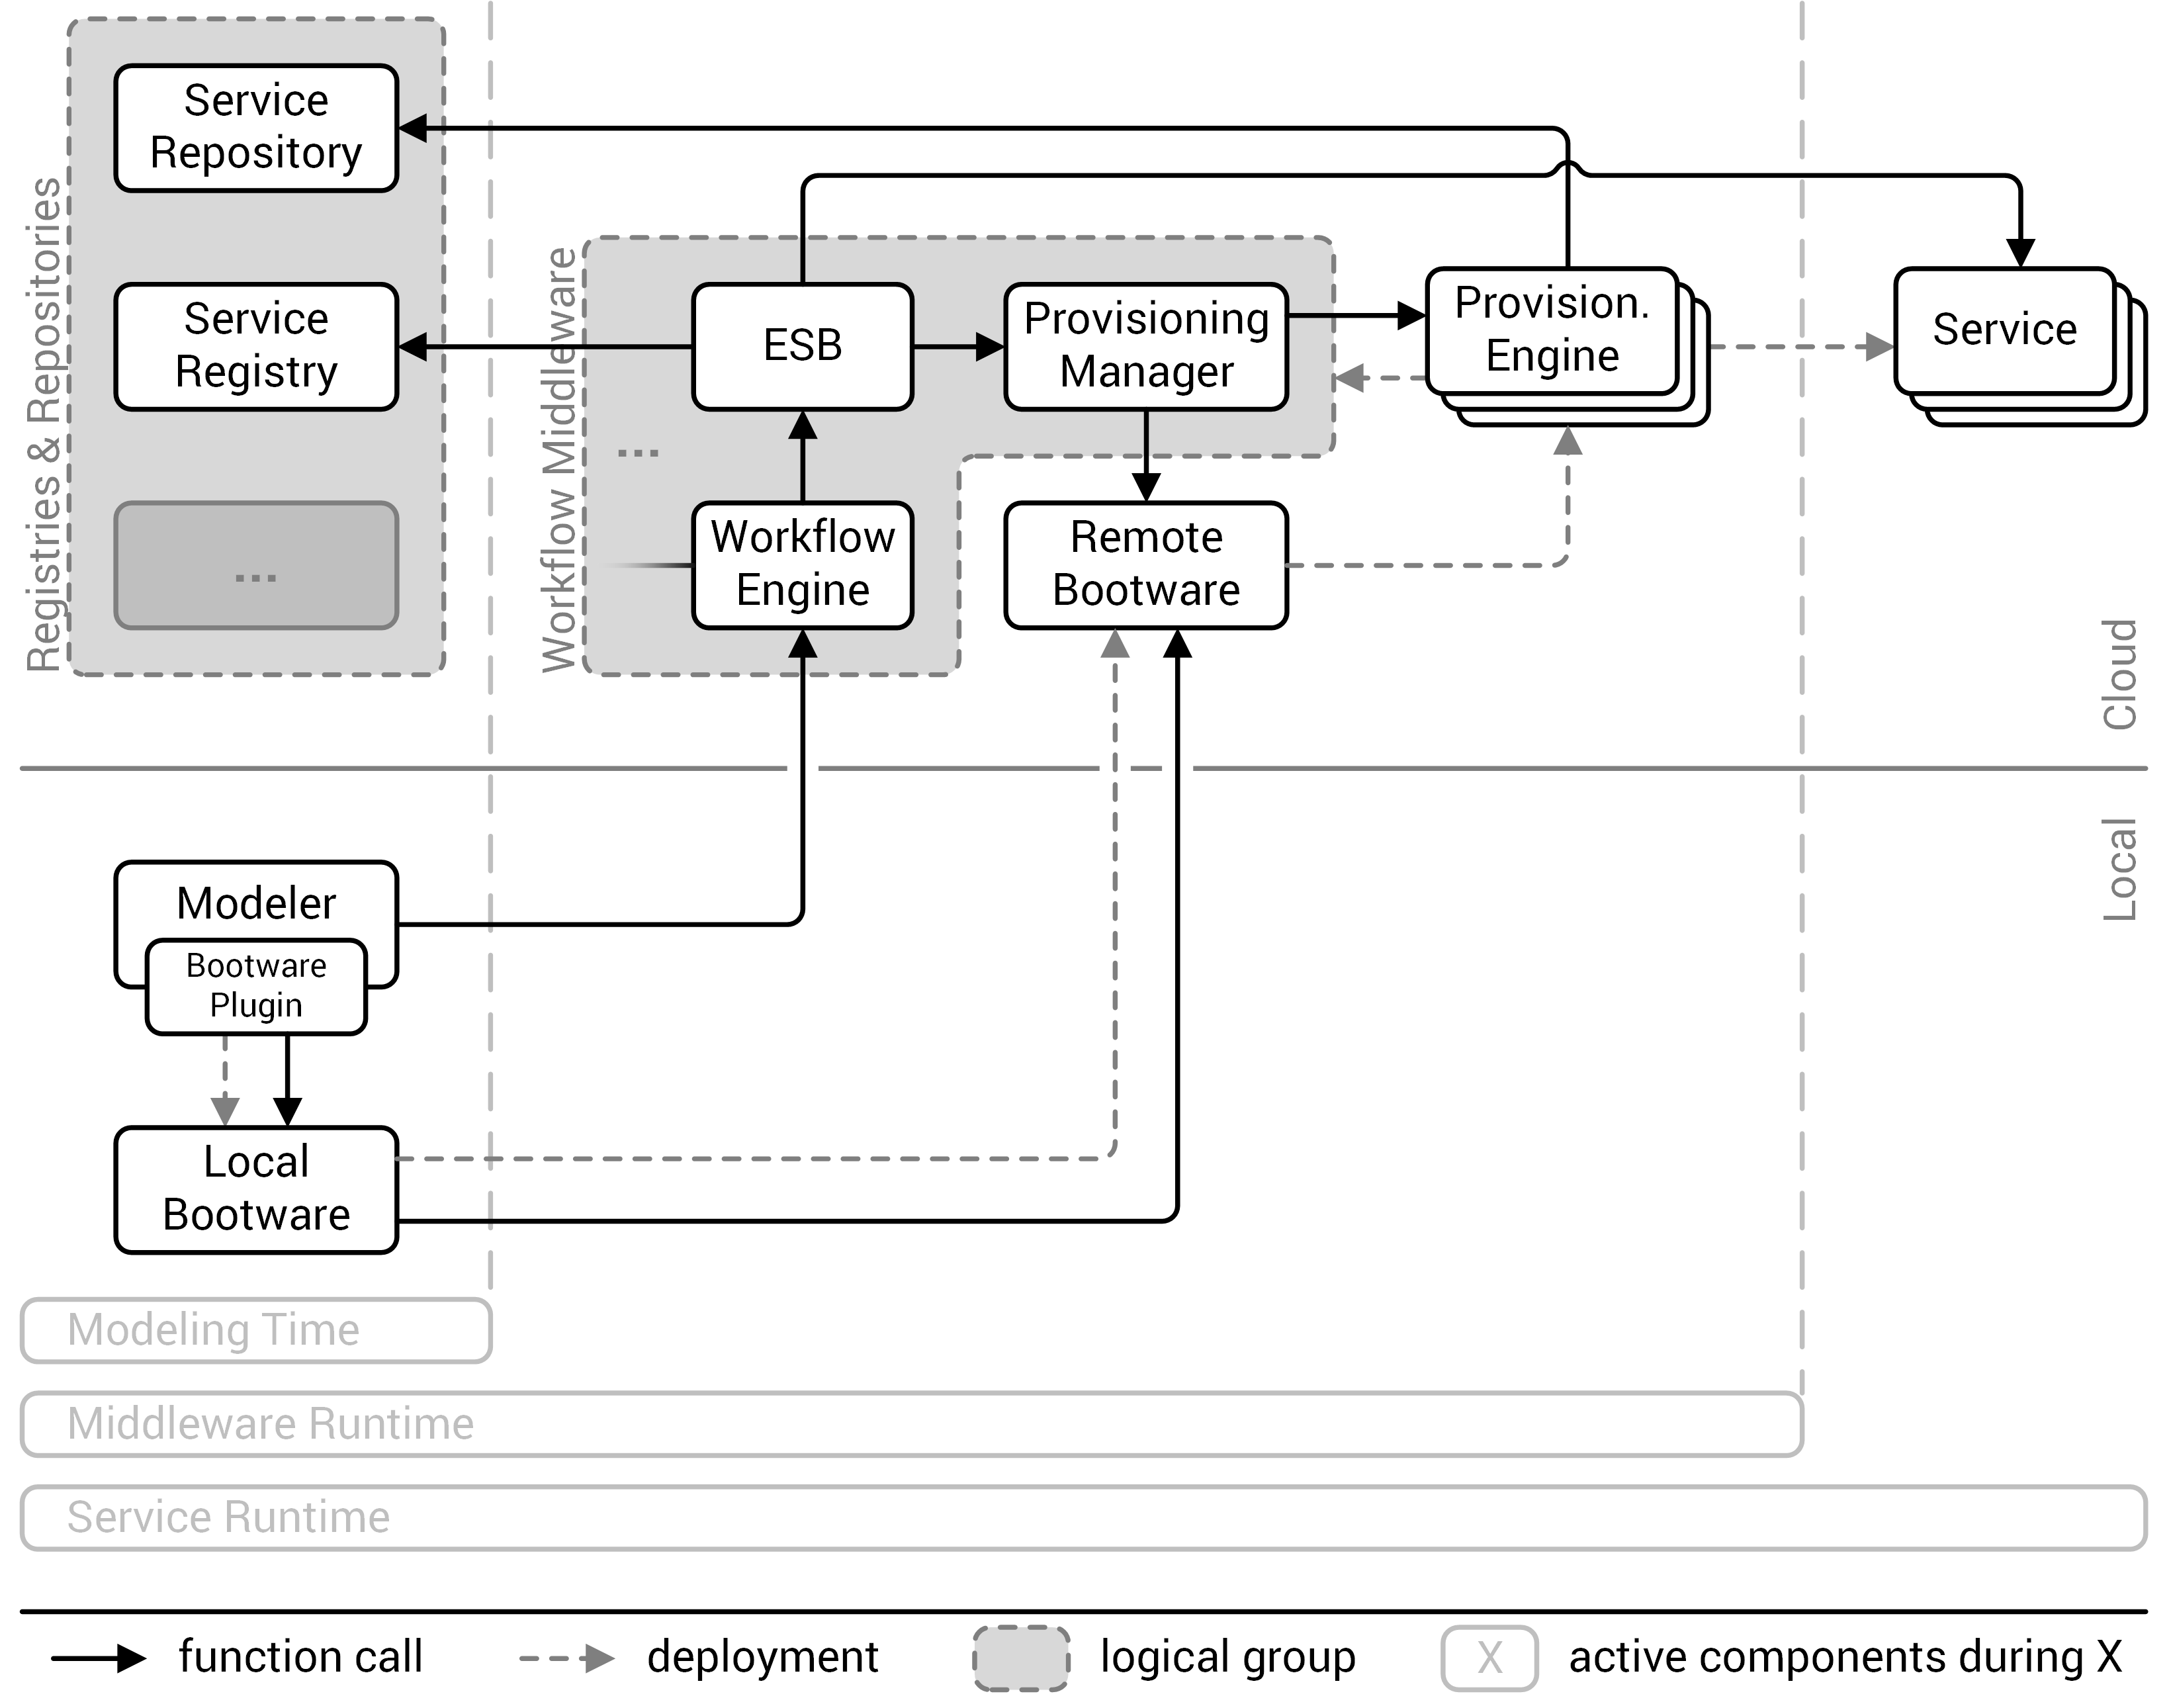
\includegraphics[resolution=600]{design/assets/modeler_plugin}
	\caption{Modeler integration with a plugin.}
	\label{image:modeler_plugin}
\end{figure}

First, the bootware adapter has to start the local bootware so that it will be in a state where it can receive and process requests.
This is shown in \autoref{image:modeler_plugin} as deployment operation from the bootware adapter to the local bootware and involves starting an executable and maybe passing along some sort of configuration file.
Once the local bootware is running, the bootware adapter has to set up the context for the following requests.
This includes telling the bootware configuration details, like the credentials for all cloud providers that will be used.
Once this is done, the modeler has to make one request to the local bootware, containing the cloud provider, the provisioning engine, and the package reference for the workflow middleware, which is shown in \autoref{image:modeler_plugin} as function call from the bootware adapter to the local bootware.
The local bootware will take this information and provision the remote bootware, which in turn will deploy a provisioning engine and the workflow middleware in the specified cloud environment.
If successful, it returns the endpoint references of the workflow middleware to the bootware adapter, which then has to set up the modeler to use these references for the actual workflow deployment.

This is the minimal work the bootware adapter has to do to kick off the bootstrapping process.
Additional functionality can be implemented if desired, but is not necessary for the core bootstrapping process.
This additional functionality could include user interface integration, additional bootware management functionality, etc.
The function call in \autoref{image:modeler_plugin} assumes that there exists some interface in the local bootware that is accessible from the outside.
In the next section we will discuss how this external communication mechanism will be implemented.
